
\documentclass[10pt]{beamer}
\usetheme{metropolis}

% ── Packages ──
\usepackage{amsmath,amssymb,amsthm}
\usepackage{tikz}
\usetikzlibrary{positioning,arrows.meta,fit,matrix,backgrounds,calc,shapes.geometric,decorations.pathreplacing}
\usepackage{graphicx}
\usepackage{array}
\usepackage{etoolbox}
\usepackage{cancel}

% ── Theorem environments ──
\theoremstyle{definition}
\newtheorem{defi}{Definition}[section]
\newtheorem{prop}{Proposition}[section]
\newtheorem{thm}{Theorem}[section]
\newtheorem{cor}{Corollary}[section]

% Custom theorem styles with colors
\setbeamercolor{block title}{bg=red!75!black,fg=white}
\setbeamercolor{block body}{bg=yellow!10!white}

\AtBeginEnvironment{prop}{%
  \setbeamercolor{block title}{bg=yellow!75!black,fg=black}%
  \setbeamercolor{block body}{bg=yellow!10!white}%
}
\AtEndEnvironment{prop}{%
  \setbeamercolor{block title}{bg=red!75!black,fg=white}%
}

\AtBeginEnvironment{thm}{%
  \setbeamercolor{block title}{bg=yellow!75!black,fg=black}%
  \setbeamercolor{block body}{bg=yellow!10!white}%
}
\AtEndEnvironment{thm}{%
  \setbeamercolor{block title}{bg=red!75!black,fg=white}%
}

\AtBeginEnvironment{cor}{%
  \setbeamercolor{block title}{bg=yellow!75!black,fg=black}%
  \setbeamercolor{block body}{bg=yellow!10!white}%
}
\AtEndEnvironment{cor}{%
  \setbeamercolor{block title}{bg=red!75!black,fg=white}%
}

% ── Highlighting ──
\newcommand{\x}[1]{\alert{\textbf{#1}}}

% ── Color shortcuts ──
\newcommand{\rd}[1]{{\color{red!70!black}#1}}
\newcommand{\bl}[1]{{\color{blue!70!black}#1}}
\newcommand{\gn}[1]{{\color{green!60!black}#1}}

% ── Cross-filling colors (matching L08/L09) ──
\newcommand{\pvt}[1]{{\color{red!70!black}\textbf{#1}}}
\newcommand{\crs}[1]{{\color{blue!70!black}#1}}

\title{Lecture 16: Eigenspaces and Diagonalization}
\subtitle{MATH203 Applied Linear Algebra}
\date{Updated May 6, 2026}
\titlegraphic{}

\begin{document}
\maketitle


% ┌─────────────────────────────────────────────────────────────────────┐
% │ SECTION-LEVEL ADR: WHAT DOES $P_i$ PROJECT ONTO?                   │
% │                                                                    │
% │ THE MACRO DESIGN: COLUMN-SPACE-FIRST DISCOVERY                    │
% │                                                                    │
% │ The audience enters knowing spectral decomposition from L15:       │
% │   A = lambda_1 P_1 + lambda_2 P_2, value table method, A^n.       │
% │ L15's last frame promised: "What subspace does each P_i project    │
% │ onto? These subspaces are the eigenspaces of A."                   │
% │                                                                    │
% │ This section delivers on that promise using a NEW 2x2 example     │
% │ (A with eigenvalues 1,3) built via the LU determinant-1 trick.    │
% │ The 2x2 setting keeps arithmetic transparent and allows genuine   │
% │ 2D geometry: eigenspace LINES through the origin, parallelogram   │
% │ decomposition visible on the page.                                │
% │                                                                    │
% │ Phase 1 -- RECALL (Frame 1): State the standing assumption.        │
% │   Never ask the audience to remember -- show everything.           │
% │                                                                    │
% │ Phase 2 -- NEW EXAMPLE (Frame 2): Introduce A, eigenvalues,       │
% │   projections P_1, P_3 with value tables and underbrace.           │
% │                                                                    │
% │ Phase 3 -- DECOMPOSE (Frames 3-4): Pick v=(2,3), split it.        │
% │   Compute P_1 v, P_3 v explicitly. Show they sum to v.            │
% │   TikZ 2D diagram: v as sum of 2 colored pieces on eigenspace     │
% │   lines, parallelogram construction with dashed lines.            │
% │                                                                    │
% │ Phase 4 -- ACT (Frames 5-6): Apply A to each piece.               │
% │   The discovery: A just SCALES each piece by lambda_i.            │
% │   Side-by-side before/after 2D TikZ with parallelogram.           │
% │                                                                    │
% │ Phase 5 -- VALUE TABLE PROOF (Frames 7-8): Why AP_i = lambda_i P_i│
% │   Use value tables -- the tool they trust from L15.                │
% │   NOT algebraic expansion. Value table is everything.              │
% │                                                                    │
% │ Phase 6 -- DEFINITION (Frames 9-10): Eigenspace = Col(P_i).       │
% │   The definition arrives AFTER the audience has seen it work.      │
% │                                                                    │
% │ LU CONSTRUCTION OF THIS EXAMPLE:                                   │
% │   L = [1 0; 1 1], U = [1 1; 0 1], P = LU = [1 1; 1 2]           │
% │   det(P) = 1, P^{-1} = [2 -1; -1 1]                              │
% │   D = diag(1,3), A = PDP^{-1} = [-1 2; -4 5]                     │
% │   det(tI-A) = (t-1)(t-3)                                          │
% │   P_1 = (A-3I)/(1-3) = [2 -1; 2 -1], value table (1,0)           │
% │   P_3 = (A-I)/(3-1) = [-1 1; -2 2], value table (0,1)            │
% │   E_1 = Col(P_1) = span{(1,1)^T}: A(1,1)^T = 1*(1,1)^T          │
% │   E_3 = Col(P_3) = span{(1,2)^T}: A(1,2)^T = 3*(1,2)^T          │
% │   Test v = (2,3): P_1 v = (1,1), P_3 v = (1,2), sum = (2,3)     │
% └─────────────────────────────────────────────────────────────────────┘
\section{What Does $P_i$ Project Onto?}


% ADR: State the standing assumption ONCE, at the very start.
% The audience needs to know the ground rules before we build anything.
% This echoes L15's assumption but makes it explicit for this lecture.
% AUDIENCE EMOTION: grounding -- "ok, same setup as last time"
% AUDIENCE ATTENTION: brief, then we move to the real content.
\begin{frame}[shrink=5]{Standing Assumption}

Throughout this lecture:

\vfill

$$\det(tI - A) = (t - \lambda_1)(t - \lambda_2)\cdots(t - \lambda_m), \qquad \lambda_i \;\text{all distinct}$$

\vfill

Same assumption as Lecture 15.

\vfill

We have the spectral decomposition:

$$A = \lambda_1 P_1 + \lambda_2 P_2 + \cdots + \lambda_m P_m$$

where $P_1, \ldots, P_m$ are compatible projections that partition $I$.

\end{frame}


\begin{frame}{Today's Question}

\vfill

Each $P_i$ is a projection: $P_i^2 = P_i$.

\vfill

Every projection projects \x{onto} some subspace --- its column space $\operatorname{Col}(P_i)$.

\vfill

$$\mathbf{v} = P_1 \mathbf{v} + P_2\mathbf{v} + \cdots + P_m\mathbf{v}$$

$$P_i\mathbf{v} \in \operatorname{Col}(P_i)$$

\vfill\pause

\begin{center}
{\Large \x{What is $\operatorname{Col}(P_i)$?}}

\vspace{0.6cm}

{\Large What does $A$ do to vectors in $\operatorname{Col}(P_i)$?}
\end{center}

\vfill

\end{frame}


% ADR: Introduce a NEW 2x2 running example, built from the LU trick.
% 2x2 keeps all arithmetic transparent -- students can verify every
% step mentally. The eigenvalues 1 and 3 give clean spectral projections
% via the Lagrange formula (divide by 1-3 = -2 and 3-1 = 2).
%
% Underbrace convention: matrix on top, name/explanation underneath.
% Value tables shown inline with the projections so the audience
% immediately connects P_i to its value table identity.
%
% AUDIENCE EMOTION: "new example, but I know the method from L15"
% AUDIENCE ATTENTION: the 2x2 format is visually compact, low cognitive
% load -- they focus on the IDEAS not the arithmetic.
\begin{frame}[shrink=5]{A New Example}

$$\underbrace{A = \begin{pmatrix}-1&2\\-4&5\end{pmatrix}}_{\text{our running example}}, \qquad \det(tI - A) = (t-1)(t-3)$$

\vfill

Eigenvalues: $\lambda_1 = 1$, $\lambda_2 = 3$.

\vfill\pause

\x{Spectral projections} (Lagrange formula from L15):

$$P_1 = \frac{A - 3I}{1 - 3} = \begin{pmatrix}2&-1\\2&-1\end{pmatrix}, \qquad
P_3 = \frac{A - I}{3 - 1} = \begin{pmatrix}-1&1\\-2&2\end{pmatrix}$$

\vfill

\x{Value tables} (from L15):

\begin{center}
\renewcommand{\arraystretch}{1.3}
\begin{tabular}{c|cc}
 & $t = 1$ & $t = 3$ \\
\hline
$A$ & $1$ & $3$ \\
$P_1$ & $\x{1}$ & $0$ \\
$P_3$ & $0$ & $\x{1}$
\end{tabular}
\end{center}

\vfill

$$A = \underbrace{1}_{\lambda_1} \cdot P_1 + \underbrace{3}_{\lambda_2} \cdot P_3$$

\end{frame}


% ADR: Pick a test vector and compute what each projection does to it.
% v = (2,3) is chosen so that BOTH pieces P_1 v and P_3 v are nonzero
% with clean integer entries: P_1 v = (1,1), P_3 v = (1,2).
%
% The explicit 2x2 matrix-vector multiplications are shown so students
% can follow each step. The sum P_1 v + P_3 v = v is the concrete
% meaning of P_1 + P_3 = I.
%
% AUDIENCE EMOTION: "oh, every vector really does split into 2 pieces"
% AUDIENCE ATTENTION: concrete numbers they can verify in their heads.
\begin{frame}{What Does $P_i$ Do to a Vector?}

Pick $\mathbf{v} = \begin{pmatrix}2\\3\end{pmatrix}$. \quad Apply each projection:

\vfill

$$\bl{P_1 \mathbf{v}} = \begin{pmatrix}2&-1\\2&-1\end{pmatrix}\begin{pmatrix}2\\3\end{pmatrix} = \bl{\begin{pmatrix}1\\1\end{pmatrix}}$$

\vfill

$$\rd{P_3 \mathbf{v}} = \begin{pmatrix}-1&1\\-2&2\end{pmatrix}\begin{pmatrix}2\\3\end{pmatrix} = \rd{\begin{pmatrix}1\\2\end{pmatrix}}$$

\vfill\pause

Check: $\;\bl{\begin{pmatrix}1\\1\end{pmatrix}} + \rd{\begin{pmatrix}1\\2\end{pmatrix}} = \begin{pmatrix}2\\3\end{pmatrix} = \mathbf{v}\;\;\checkmark$

\end{frame}


% ADR: Show the decomposition geometrically in 2D.
% This is the VISUAL ANCHOR for the rest of the section.
%
% Eigenspace lines E_1 = span{(1,1)} and E_3 = span{(1,2)} through
% the origin. P_1 v = (1,1) lies on E_1, P_3 v = (1,2) lies on E_3.
% Dashed parallelogram construction: from P_1 v to v, from P_3 v to v.
%
% All vectors start from the origin. The parallelogram shows that
% v = P_1 v + P_3 v geometrically.
%
% AUDIENCE EMOTION: satisfaction -- "the pieces add up on the picture"
% AUDIENCE ATTENTION: the 2D diagram is the mental image they carry
% through the rest of the lecture.
\begin{frame}[shrink=5]{Every Vector Splits Into Eigenspace Pieces}

$$\mathbf{v} \;=\; \bl{P_1 \mathbf{v}} \;+\; \rd{P_3 \mathbf{v}} \;=\; \bl{\begin{pmatrix}1\\1\end{pmatrix}} + \rd{\begin{pmatrix}1\\2\end{pmatrix}} \;=\; \begin{pmatrix}2\\3\end{pmatrix} \;\checkmark$$

\vfill

\begin{center}
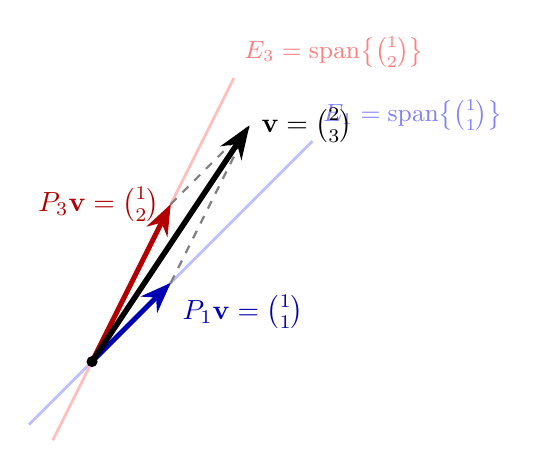
\begin{tikzpicture}[>=Stealth, scale=1.0]
  % Eigenspace lines through origin
  \draw[blue!25, line width=1pt] (-0.8,-0.8) -- (2.8,2.8)
    node[above right, blue!50, font=\small] {$E_1 = \operatorname{span}\bigl\{\binom{1}{1}\bigr\}$};
  \draw[red!25, line width=1pt] (-0.5,-1) -- (1.8,3.6)
    node[above right, red!50, font=\small] {$E_3 = \operatorname{span}\bigl\{\binom{1}{2}\bigr\}$};
  % Eigenvector components -- all from origin
  \draw[->, blue!70!black, line width=1.8pt] (0,0) -- (1,1)
    node[below right] {$\bl{P_1\mathbf{v}} = \binom{1}{1}$};
  \draw[->, red!70!black, line width=1.8pt] (0,0) -- (1,2)
    node[left] {$\rd{P_3\mathbf{v}} = \binom{1}{2}$};
  % Dashed parallelogram construction
  \draw[dashed, gray, line width=0.8pt] (1,1) -- (2,3);
  \draw[dashed, gray, line width=0.8pt] (1,2) -- (2,3);
  % v = sum
  \draw[->, black, line width=2pt] (0,0) -- (2,3)
    node[right] {$\mathbf{v} = \binom{2}{3}$};
  % Origin dot
  \fill (0,0) circle (2pt);
\end{tikzpicture}
\end{center}

\vfill

$P_1 + P_3 = I$: every vector decomposes into eigenspace pieces (parallelogram law).

\end{frame}


% ADR: THE KEY DISCOVERY -- A scales each piece by its eigenvalue.
% Compute A * (P_1 v) and A * (P_3 v) separately.
% A * (1,1)^T = (-1+2, -4+5)^T = (1,1)^T = 1 * P_1 v
% A * (1,2)^T = (-1+4, -4+10)^T = (3,6)^T = 3 * P_3 v
%
% The reveal is staged: first compute A*(P_1 v) and notice the scalar.
% Then show the other. The pattern emerges before we name it.
%
% AUDIENCE EMOTION: surprise -> recognition -- "A just scales each piece!"
% AUDIENCE ATTENTION: the 2x2 multiplication is simple enough to verify
% mentally, keeping the audience actively checking.
\begin{frame}{What Does $A$ Do to Each Piece?}

Apply $A$ to the \bl{first piece}:

\vfill

$$A \cdot \bl{P_1\mathbf{v}} = \begin{pmatrix}-1&2\\-4&5\end{pmatrix}\bl{\begin{pmatrix}1\\1\end{pmatrix}} = \begin{pmatrix}1\\1\end{pmatrix} = \x{1} \cdot \bl{P_1\mathbf{v}}$$

\vfill\pause

Apply $A$ to the \rd{second piece}:

$$A \cdot \rd{P_3\mathbf{v}} = \begin{pmatrix}-1&2\\-4&5\end{pmatrix}\rd{\begin{pmatrix}1\\2\end{pmatrix}} = \begin{pmatrix}3\\6\end{pmatrix} = \x{3} \cdot \rd{P_3\mathbf{v}}$$

\vfill\pause

\begin{center}
\fbox{\parbox{0.65\textwidth}{\centering
$A$ \x{scales each piece by its eigenvalue}: $\lambda_1 = 1$ and $\lambda_2 = 3$.
}}
\end{center}

\end{frame}


% ADR: The underbrace reveal and side-by-side before/after 2D diagrams.
% Before: v = P_1 v + P_3 v = (1,1) + (1,2) = (2,3)
% After:  Av = 1*(1,1) + 3*(1,2) = (1,1) + (3,6) = (4,7)
%
% Both diagrams use the SAME coordinate system so the stretching
% of the red piece (x3) is visually apparent. Blue piece stays the
% same length (x1). The parallelogram stretches accordingly.
%
% AUDIENCE EMOTION: "this is clean" -- the underbrace + diagram pair
% makes the pattern unmistakable.
% AUDIENCE ATTENTION: two pictures to compare, active visual processing.
\begin{frame}[shrink=10]{$A$ Scales Each Piece by Its Eigenvalue}

$$A\mathbf{v} \;=\; A\bigl(\bl{P_1\mathbf{v}} + \rd{P_3\mathbf{v}}\bigr) \;=\; \underbrace{\x{1}}_{\lambda_1} \cdot \bl{P_1\mathbf{v}} \;+\; \underbrace{\x{3}}_{\lambda_2} \cdot \rd{P_3\mathbf{v}}$$

\vfill

\begin{center}
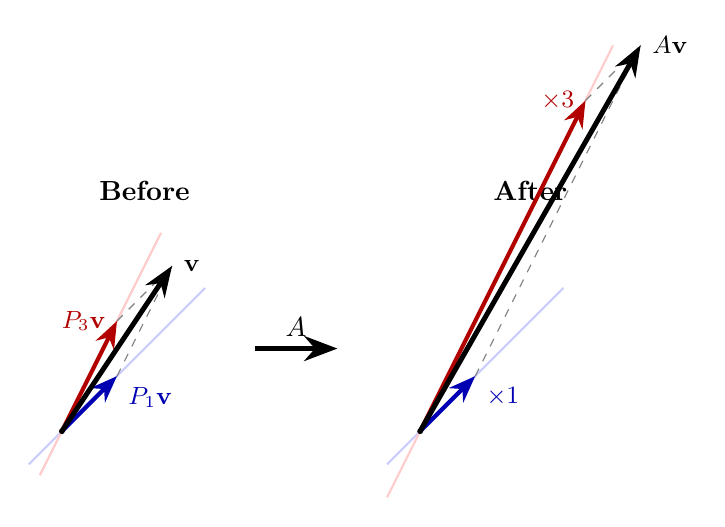
\begin{tikzpicture}[>=Stealth, scale=0.7]
  % ── BEFORE ──
  \node[above, font=\bfseries] at (1.5, 4) {Before};
  % Eigenspace lines
  \draw[blue!20, line width=0.8pt] (-0.6,-0.6) -- (2.6,2.6);
  \draw[red!20, line width=0.8pt] (-0.4,-0.8) -- (1.8,3.6);
  % Components from origin
  \draw[->, blue!70!black, line width=1.5pt] (0,0) -- (1,1)
    node[below right, font=\small] {$\bl{P_1\mathbf{v}}$};
  \draw[->, red!70!black, line width=1.5pt] (0,0) -- (1,2)
    node[left, font=\small] {$\rd{P_3\mathbf{v}}$};
  % Dashed parallelogram
  \draw[dashed, gray] (1,1) -- (2,3);
  \draw[dashed, gray] (1,2) -- (2,3);
  % v
  \draw[->, black, line width=1.8pt] (0,0) -- (2,3)
    node[right, font=\small] {$\mathbf{v}$};
  \fill (0,0) circle (1.5pt);

  % Arrow between diagrams
  \draw[->, line width=2pt] (3.5,1.5) -- node[above] {$A$} (5,1.5);

  % ── AFTER ──
  \begin{scope}[xshift=6.5cm]
  \node[above, font=\bfseries] at (2, 4) {After};
  % Eigenspace lines
  \draw[blue!20, line width=0.8pt] (-0.6,-0.6) -- (2.6,2.6);
  \draw[red!20, line width=0.8pt] (-0.6,-1.2) -- (3.5,7);
  % Scaled components from origin
  \draw[->, blue!70!black, line width=1.5pt] (0,0) -- (1,1)
    node[below right, font=\small] {$\bl{\times 1}$};
  \draw[->, red!70!black, line width=1.5pt] (0,0) -- (3,6)
    node[left, font=\small] {$\rd{\times 3}$};
  % Dashed parallelogram
  \draw[dashed, gray] (1,1) -- (4,7);
  \draw[dashed, gray] (3,6) -- (4,7);
  % Av
  \draw[->, black, line width=1.8pt] (0,0) -- (4,7)
    node[right, font=\small] {$A\mathbf{v}$};
  \fill (0,0) circle (1.5pt);
  \end{scope}
\end{tikzpicture}
\end{center}

\vfill

$A$ doesn't rotate or mix the pieces --- it \x{only scales} each one along its eigenspace.

\end{frame}


% ADR: VALUE TABLE PROOF of AP_i = lambda_i P_i.
% This is the audience's trusted tool from L15. We do NOT expand
% A(P_1) algebraically -- that would feel like "recalling hard knowledge."
% Instead we multiply value tables entry-wise.
%
% Value table of A: (1, 3).
% Value table of P_1: (1, 0).
% Product: (1*1, 3*0) = (1, 0) = value table of 1*P_1.
% Same value table -> same matrix.
%
% AUDIENCE EMOTION: "value tables make this trivial"
% AUDIENCE ATTENTION: the entry-wise multiplication is instant to verify.
\begin{frame}[shrink=15]{Why? --- Value Table Proof}

\x{Why} does $A$ scale the $P_1$-piece by $\lambda_1$?

\vfill

\x{Multiply} value tables entry-wise:

\begin{center}
\renewcommand{\arraystretch}{1.3}
\begin{tabular}{c|cc}
 & $t = 1$ & $t = 3$ \\
\hline
$A$ & $1$ & $3$ \\
$\times\; P_1$ & $1$ & $0$ \\
\hline
$AP_1$ & $\x{1}$ & $\x{0}$
\end{tabular}
\end{center}

\vfill\pause

Value table of $\lambda_1 P_1 = 1 \cdot P_1$:

\begin{center}
\renewcommand{\arraystretch}{1.3}
\begin{tabular}{c|cc}
 & $t = 1$ & $t = 3$ \\
\hline
$1 \cdot P_1$ & $\x{1}$ & $\x{0}$
\end{tabular}
\end{center}

\x{Same value table} $\implies$ \x{same matrix}: $\;\; AP_1 = \lambda_1 P_1 = 1 \cdot P_1$.

\vfill\pause

Similarly for $P_3$:

\begin{center}
\renewcommand{\arraystretch}{1.3}
\begin{tabular}{c|cc}
 & $t = 1$ & $t = 3$ \\
\hline
$A$ & $1$ & $3$ \\
$\times\; P_3$ & $0$ & $1$ \\
\hline
$AP_3$ & $\x{0}$ & $\x{3}$
\end{tabular}
$\;=\;$ value table of $3 P_3$ \;\checkmark
\end{center}

\end{frame}


% ADR: Left multiplication too -- P_i A = lambda_i P_i.
% This is quick but important: it sets up left eigenvectors in S3.
% The key point: value table multiplication is entry-wise, so order
% doesn't matter. This proves A commutes with each P_i.
%
% AUDIENCE EMOTION: "A commutes with P_i -- and the value table makes
% it obvious"
% AUDIENCE ATTENTION: short frame, one key fact, builds on previous.
\begin{frame}{$A$ Commutes With Each $P_i$}

What about $P_1 A$? \x{Multiply} value tables in the other order:

\begin{center}
\renewcommand{\arraystretch}{1.3}
\begin{tabular}{c|cc}
 & $t = 1$ & $t = 3$ \\
\hline
$P_1$ & $1$ & $0$ \\
$\times\; A$ & $1$ & $3$ \\
\hline
$P_1 A$ & $\x{1}$ & $\x{0}$
\end{tabular}
\end{center}

Same value table as $AP_1$! \quad So $P_1 A = AP_1 = \lambda_1 P_1$.

\vfill\pause

\begin{center}
\fbox{\parbox{0.85\textwidth}{\centering
Value table multiplication is \x{entry-wise}: order doesn't matter.\\[6pt]
$AP_i = P_i A = \lambda_i P_i \qquad\text{for each } i$
}}
\end{center}

\vfill

$A$ commutes with every spectral projection.

\vfill

(This fact will matter when we find \x{left eigenvectors} later.)

\end{frame}


% ADR: From AP_i = lambda_i P_i to the eigenspace definition.
% The logic: if x in Col(P_i), then P_i x = x (projection fixes its
% column space), so Ax = AP_i x = lambda_i P_i x = lambda_i x.
% Every vector in Col(P_i) is just scaled by lambda_i.
%
% This is the bridge from "what P_i does" to "what eigenspace means."
%
% AUDIENCE EMOTION: "so Col(P_i) is where A just multiplies by lambda_i"
% AUDIENCE ATTENTION: the chain Ax = AP_ix = lambda_iP_ix = lambda_ix
% is short and each step has a reason shown explicitly.
\begin{frame}{From $AP_i = \lambda_i P_i$ to Eigenvectors}

Suppose $\mathbf{x} \in \operatorname{Col}(P_i)$.

\vfill

Since $P_i$ is a projection, it \x{fixes} its own column space: $P_i\mathbf{x} = \mathbf{x}$.

\vfill\pause

Then:

$$A\mathbf{x} = A \underbrace{P_i \mathbf{x}}_{= \mathbf{x}} = \underbrace{AP_i}_{= \lambda_i P_i}\mathbf{x} = \lambda_i \underbrace{P_i\mathbf{x}}_{= \mathbf{x}} = \lambda_i \mathbf{x}$$

\vfill

Every vector in $\operatorname{Col}(P_i)$ is scaled by $\lambda_i$.

\vfill\pause

\begin{center}
\fbox{\parbox{0.75\textwidth}{\centering
$\operatorname{Col}(P_i)$ = the subspace where $A$ acts as\\[4pt]
\x{scalar multiplication by $\lambda_i$}.
}}
\end{center}

\end{frame}


% ADR: The eigenspace definition. We define it as Col(P_i) FIRST,
% then give the equivalent {x : Ax = lambda x} form.
%
% Then verify on the running 2x2 example: find a basis for each
% Col(P_i) and check that A scales it by the right eigenvalue.
%
% Col(P_1) = span{(1,1)^T}: first column of P_1 = (2,2)^T ~ (1,1)^T
% Check: A(1,1)^T = (-1+2, -4+5)^T = (1,1)^T = 1*(1,1)^T
%
% Col(P_3) = span{(1,2)^T}: second column of P_3 = (1,2)^T
% Check: A(1,2)^T = (-1+4, -4+10)^T = (3,6)^T = 3*(1,2)^T
%
% AUDIENCE EMOTION: "so THAT's what an eigenspace is"
% AUDIENCE ATTENTION: two quick checks -- each is one line of
% 2x2 arithmetic the audience can do in their head.
\begin{frame}{The Eigenspace}

\begin{defi}[Eigenspace]
The \x{eigenspace} of $A$ for eigenvalue $\lambda_i$ is
$$E_{\lambda_i} \;=\; \bigl\{\,\mathbf{x} \in \mathbb{R}^n : A\mathbf{x} = \lambda_i \mathbf{x}\,\bigr\}$$
\end{defi}

\vfill

The set of all vectors that $A$ simply \x{scales} by $\lambda_i$.

\vfill

\begin{prop}
$E_{\lambda_i} = \operatorname{Col}(P_i)$ \quad (the column space of the spectral projection).
\end{prop}

\vfill

\textit{Proof on next slide.}

\end{frame}

\begin{frame}{Proof: $E_{\lambda_i} = \operatorname{Col}(P_i)$}

Proof ($\supseteq$): If $\mathbf{x} \in \operatorname{Col}(P_i)$, then $P_i\mathbf{x} = \mathbf{x}$ (projection fixes its column space), so

$$A\mathbf{x} = A P_i\mathbf{x} = \lambda_i P_i\mathbf{x} = \lambda_i\mathbf{x} \quad\implies\quad \mathbf{x} \in E_{\lambda_i}$$

\vfill\pause

Proof ($\subseteq$): $P_i$ is a \x{polynomial} of $A$ (Lagrange interpolation formula from L15).

\smallskip

For any polynomial $f$ of $A$: if $A\mathbf{x} = \lambda_i\mathbf{x}$, then $f(A)\mathbf{x} = f(\lambda_i)\mathbf{x}$.

\smallskip

Since $P_i$ is the Lagrange polynomial that evaluates to \x{$1$} at $\lambda_i$:

$$P_i\mathbf{x} = 1 \cdot \mathbf{x} = \mathbf{x} \quad\implies\quad \mathbf{x} \in \operatorname{Col}(P_i) \qed$$

\end{frame}


\begin{frame}{Check on Our Example}

$E_1 = \operatorname{Col}(P_1) = \operatorname{span}\left\{\begin{pmatrix}1\\1\end{pmatrix}\right\}$. \quad
$A\begin{pmatrix}1\\1\end{pmatrix} = \begin{pmatrix}1\\1\end{pmatrix} = \x{1}\begin{pmatrix}1\\1\end{pmatrix}$ \;\checkmark

\vfill

$E_3 = \operatorname{Col}(P_3) = \operatorname{span}\left\{\begin{pmatrix}1\\2\end{pmatrix}\right\}$. \quad
$A\begin{pmatrix}1\\2\end{pmatrix} = \begin{pmatrix}3\\6\end{pmatrix} = \x{3}\begin{pmatrix}1\\2\end{pmatrix}$ \;\checkmark

\vfill\pause

\begin{center}
\fbox{\parbox{0.75\textwidth}{\centering
The eigenspace $E_{\lambda_i}$ is \x{exactly} the column space of $P_i$.\\[4pt]
The spectral projections \x{project onto} the eigenspaces.
}}
\end{center}

\end{frame}


% ADR: Section summary -- crystallize the key insight before moving on.
% One big statement, no clutter.
%
% AUDIENCE EMOTION: "I understand what eigenspaces ARE now -- they're
% where A just multiplies"
% AUDIENCE ATTENTION: one-line summary, then scene change.
\begin{frame}{}

\vfill

\begin{center}
{\Large $P_i$ projects onto $E_{\lambda_i}$:}

\vspace{0.8cm}

{\Large the subspace where $A$ acts as}

\vspace{0.8cm}

{\Large \x{scalar multiplication by $\lambda_i$}.}
\end{center}

\vfill

\end{frame}


% ┌─────��────────────────────────────────────────��──────────────────────┐
% │ SECTION-LEVEL ADR: COMPATIBLE PROJECTIONS REVISITED                │
% │                                                                    │
% │ The audience saw compatible projections in L08 and value tables in │
% │ L15. This section uses value tables on the 2x2 example to:        │
% │   1. Re-verify P_i^2 = P_i (projections)                          │
% │   2. Verify P_1 P_3 = 0 (compatibility)                           │
% ���   3. Verify P_1 + P_3 = I (partition)                             │
% │   4. Prove eigenvectors from different eigenspaces are independent │
% │   5. State the big picture: eigenspaces span R^n                  │
% │                                                                    │
% │ All value tables in PROPER TABULAR FORMAT, never tuple notation.   │
% └───────��────────────────────────────────���────────────────────────────┘
\section{Compatible Projections Revisited}


% ADR: Value table checks for projection property.
% Square each entry: if same, it's a projection.
% AUDIENCE EMOTION: "value tables make this instant"
% AUDIENCE ATTENTION: two tables side by side, scannable.
\begin{frame}[shrink=5]{Recall: Where Did $P_1, P_3$ Come From?}

In Lecture 15, we plugged $A$ into the \x{Lagrange interpolation polynomials}:

$$P_1 = \frac{A - 3I}{1 - 3}, \qquad P_3 = \frac{A - I}{3 - 1}$$

This gave the \x{spectral decomposition}: $A = 1 \cdot P_1 + 3 \cdot P_3$.

\vfill

Their \x{value tables} (from Lecture 15):

\begin{center}
\renewcommand{\arraystretch}{1.3}
\begin{tabular}{c|cc}
 & $t = 1$ & $t = 3$ \\
\hline
$P_1$ & $1$ & $0$ \\
$P_3$ & $0$ & $1$
\end{tabular}
\end{center}

\vfill\pause

We \x{claimed} $P_1, P_3$ are compatible projections that partition $I$.

\vfill

Let's verify this using value tables --- the tool we trust from Lecture 15.

\end{frame}


\begin{frame}{Are $P_1, P_3$ Projections?}

Check with value tables --- \x{square each entry}:

\vfill

\begin{center}
\renewcommand{\arraystretch}{1.3}
\begin{tabular}{c|cc}
 & $t = 1$ & $t = 3$ \\
\hline
$P_1$ & $1$ & $0$ \\
$P_1^2$ & $1^2 = \x{1}$ & $0^2 = \x{0}$
\end{tabular}
\qquad\qquad
\begin{tabular}{c|cc}
 & $t = 1$ & $t = 3$ \\
\hline
$P_3$ & $0$ & $1$ \\
$P_3^2$ & $0^2 = \x{0}$ & $1^2 = \x{1}$
\end{tabular}
\end{center}

\vfill

Same value tables $\implies$ $P_1^2 = P_1$ and $P_3^2 = P_3$. \quad Both are \x{projections}. \;\checkmark

\end{frame}


% ADR: Compatibility (P_1P_3 = 0) and partition (P_1+P_3 = I).
% Both are instant from value tables.
% AUDIENCE EMOTION: "so fast compared to multiplying matrices"
% AUDIENCE ATTENTION: two checks, clean tabular format.
\begin{frame}[shrink=5]{Compatible? Partition of $I$?}

\x{Compatible?} Multiply value tables entry-wise:

\begin{center}
\renewcommand{\arraystretch}{1.3}
\begin{tabular}{c|cc}
 & $t = 1$ & $t = 3$ \\
\hline
$P_1$ & $1$ & $0$ \\
$\times\; P_3$ & $0$ & $1$ \\
\hline
$P_1 P_3$ & $\x{0}$ & $\x{0}$
\end{tabular}
\end{center}

Value table all zeros $\implies$ $P_1 P_3 = 0$. \quad \x{Compatible!} \;\checkmark

\vfill\pause

\x{Partition of $I$?} Add value tables:

\begin{center}
\renewcommand{\arraystretch}{1.3}
\begin{tabular}{c|cc}
 & $t = 1$ & $t = 3$ \\
\hline
$P_1$ & $1$ & $0$ \\
$+\; P_3$ & $0$ & $1$ \\
\hline
$P_1 + P_3$ & $\x{1}$ & $\x{1}$
\end{tabular}
\end{center}

Value table $= $ value table of $I$. \quad $P_1 + P_3 = I$. \;\checkmark

\end{frame}


% ADR: Connect back to L08's compatible projection theory.
% The value table method AUTOMATICALLY produces compatible projections.
% AUDIENCE EMOTION: "the machinery is self-consistent"
% AUDIENCE ATTENTION: boxed key insight.
\begin{frame}[shrink=5]{Connection to Lecture 8: Compatible Projections}

From Lecture 8: $P_1 P_3 = 0$ means $\operatorname{Col}(P_3) \subset \operatorname{Null}(P_1)$ and $\operatorname{Col}(P_1) \subset \operatorname{Null}(P_3)$.

\vfill

\begin{center}
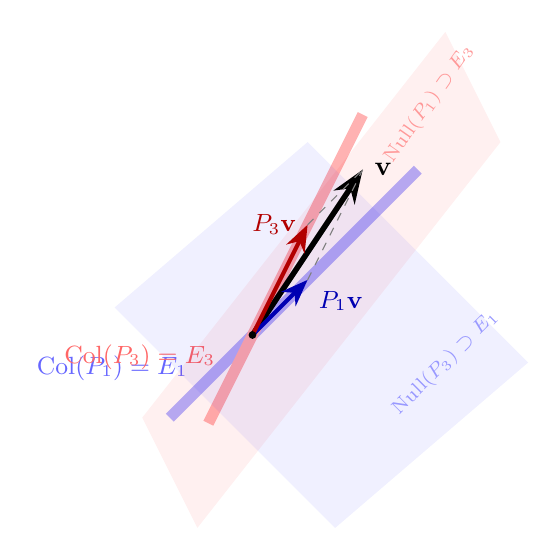
\begin{tikzpicture}[>=Stealth, scale=0.7]
  % Eigenspace lines as column spaces
  \draw[blue!30, line width=4pt] (-1.5,-1.5) -- (3,3);
  \node[blue!60, above left, font=\small] at (-1,-1) {$\operatorname{Col}(P_1) = E_1$};
  \draw[red!30, line width=4pt] (-0.8,-1.6) -- (2,4);
  \node[red!60, above left, font=\small] at (-0.5,-0.8) {$\operatorname{Col}(P_3) = E_3$};
  % Null space shading
  \fill[red, opacity=0.06] (-2,-1.5) -- (3.5,5.5) -- (4.5,3.5) -- (-1,-3.5) -- cycle;
  \node[red!40, font=\scriptsize, rotate=55] at (3.2,4.2) {$\operatorname{Null}(P_1) \supset E_3$};
  \fill[blue, opacity=0.06] (-2.5,0.5) -- (1.5,-3.5) -- (5,-0.5) -- (1,3.5) -- cycle;
  \node[blue!40, font=\scriptsize, rotate=45] at (3.5,-0.5) {$\operatorname{Null}(P_3) \supset E_1$};
  % Vector and projections
  \draw[->, black, line width=2pt] (0,0) -- (2,3) node[right] {$\mathbf{v}$};
  \draw[->, blue!70!black, line width=1.5pt] (0,0) -- (1,1) node[below right, font=\small] {$P_1\mathbf{v}$};
  \draw[->, red!70!black, line width=1.5pt] (0,0) -- (1,2) node[left, font=\small] {$P_3\mathbf{v}$};
  \draw[dashed, gray] (1,1) -- (2,3);
  \draw[dashed, gray] (1,2) -- (2,3);
  \fill (0,0) circle (2pt);
\end{tikzpicture}
\end{center}

\vfill

Each eigenspace lives inside the null space of the \x{other} projection.

\vfill\pause

\begin{center}
\fbox{\parbox{0.85\textwidth}{\centering
The Lagrange formula from L15 \x{automatically}\\[4pt]
produces compatible projections.\\[6pt]
No extra verification needed --- it's built into the construction.
}}
\end{center}

\end{frame}


% ADR: THE theorem on linear independence of eigenvectors.
% This is a SERIOUS theorem, stated in full generality for m
% eigenvectors with m distinct eigenvalues.
% Proof uses spectral projections: P_i kills eigenvectors from
% other eigenspaces (because the Lagrange formula for P_i contains
% the factor (A - lambda_j I)), and P_i fixes its own eigenspace.
% Apply P_i to the linear combination: all terms except the i-th vanish.
%
% Legacy slides (SpectralDecompositionForRepeatedRoots.tex, line 852)
% state this as a theorem with this exact proof technique.
%
% AUDIENCE EMOTION: "a powerful theorem with a clean proof"
% AUDIENCE ATTENTION: the proof is short but the theorem is general.
\begin{frame}[shrink=5]{Eigenvectors With Different Eigenvalues Are Independent}

From Lecture 9, Proposition (Independent Decompositions):

\vfill

\begin{center}
\fbox{\parbox{0.88\textwidth}{
For a compatible family $\{P_1, \ldots, P_m\}$, the nonzero vectors among $\{P_1\mathbf{v}, \ldots, P_m\mathbf{v}\}$ are \x{linearly independent}.\\[4pt]
{\small Proof: multiply both sides of $\sum c_i P_i\mathbf{v} = 0$ by $P_j$. Since $P_jP_i = 0$ for $j \neq i$, only the $j$-th term survives: $c_j P_j\mathbf{v} = 0$.}
}}
\end{center}

\vfill\pause

Since the spectral projections $P_1, \ldots, P_m$ are compatible:

\begin{cor}
Let $\mathbf{v}_1, \ldots, \mathbf{v}_m$ be eigenvectors of $A$ with \x{distinct} eigenvalues $\lambda_1, \ldots, \lambda_m$. Then $\mathbf{v}_1, \ldots, \mathbf{v}_m$ are \x{linearly independent}.
\end{cor}

\vfill

Each $\mathbf{v}_i \in E_{\lambda_i} = \operatorname{Col}(P_i)$, so $P_i\mathbf{v}_i = \mathbf{v}_i \neq 0$ and $P_j\mathbf{v}_i = 0$ for $j \neq i$.

The Lecture 9 proposition applies directly. \qed

\end{frame}


% ADR: Unique decomposition -- callback to L09.
% L09 proved: compatible projections that partition P give unique
% decomposition of every vector in Col(P). Here P_1 + P_3 = I,
% so Col(I) = R^n -- EVERY vector decomposes uniquely.
% DO NOT use direct sum notation (oplus) -- students haven't learned it
% (L09 explicitly says "we will not use this notation").
% AUDIENCE EMOTION: "the whole space is covered"
% AUDIENCE ATTENTION: callback to L09, then boxed statement.
\begin{frame}{Unique Decomposition (Lecture 9 Callback)}

From Lecture 9: compatible projections that partition $I$ give a \x{unique decomposition} of every vector.

\vfill

Since $P_1 + P_3 = I$, every $\mathbf{v} \in \mathbb{R}^n$ decomposes as:

$$\mathbf{v} = \underbrace{P_1\mathbf{v}}_{\in\, E_1} + \underbrace{P_3\mathbf{v}}_{\in\, E_3}$$

and by the corollary above, this decomposition is \x{unique}.

\vfill

\begin{center}
\fbox{\parbox{0.85\textwidth}{\centering
The eigenspaces $E_{\lambda_1}, \ldots, E_{\lambda_m}$ together \x{span} all of $\mathbb{R}^n$.\\[6pt]
Every vector decomposes \x{uniquely} into eigenvector pieces.\\[6pt]
{\small (This is the geometric meaning of $P_1 + P_2 + \cdots + P_m = I$.)}
}}
\end{center}

\end{frame}


% ┌─────��───────────────────────────────────────────────────────────────┐
% │ SECTION-LEVEL ADR: CROSS-FILLING SPECTRAL PROJECTIONS              ��
% │                                                                    │
% │ The 2x2 running example has only rank-1 projections, so cross-     │
% │ filling is trivial. To show a GENUINE two-step cross-fill, we      │
% │ introduce a 3x3 example B with a repeated eigenvalue:              │
% │                                                                    │
% │   B = [[2,0,3],[0,2,3],[0,0,5]], eigenvalues 2,2,5                │
% │   det(tI-B) = (t-2)^2(t-5)                                        │
% │   min poly = (t-2)(t-5) -- distinct factors, everything works      │
% │                                                                    │
% │   P_5 = (B-2I)/3 = [[0,0,1],[0,0,1],[0,0,1]] (rank 1)            │
% │   P_2 = I - P_5 = [[1,0,-1],[0,1,-1],[0,0,0]] (rank 2)           │
% │                                                                    │
% │ Cross-fill P_2 (two steps):                                        │
% │   Pivot (1,1)=1: col=(1,0,0)^T, row=(1,0,-1)                     │
% │   Remainder pivot (2,2)=1: col=(0,1,0)^T, row=(0,1,-1)           │
% │   U_2 = [[1,0],[0,1],[0,0]], V_2 = [[1,0,-1],[0,1,-1]]           │
% │                                                                    │
% │ Cross-fill P_5 (one step):                                        │
% │   Pivot (3,3)=1: col=(1,1,1)^T, row=(0,0,1)                      │
% │   U_5 = (1,1,1)^T, V_5 = (0,0,1)                                 │
% │                                                                    │
% │ Right eigenvectors = columns of U_i                                │
% │ Left eigenvectors = rows of V_i                                    │
% │ Cross-eigenspace: V_2 U_5 = 0, V_5 U_2 = 0                       │
% └─────────────────────────────────────���───────────────────────────────┘
\section{Cross-Filling the Spectral Projections}


% ADR: Introduce a 3x3 example with a repeated eigenvalue.
% B is upper triangular so eigenvalues are visible, but the spectral
% machinery works without using that. The repeated eigenvalue 2 gives
% a rank-2 projection P_2 that requires genuine cross-filling.
%
% AUDIENCE EMOTION: "repeated eigenvalue? will our method still work?"
% AUDIENCE ATTENTION: new example, slight tension about the repeated root.
\begin{frame}[shrink=5]{A New Example --- Repeated Eigenvalue}

$$\underbrace{B = \begin{pmatrix}2&0&3\\0&2&3\\0&0&5\end{pmatrix}}_{\text{eigenvalues } 2, 2, 5}, \qquad \det(tI - B) = (t-2)^2(t-5)$$

\vfill

Two \x{distinct} eigenvalues: $\lambda_1 = 2$, $\lambda_2 = 5$.

\vfill\pause

\x{Spectral projections} (Lagrange formula):

$$P_5 = \frac{B - 2I}{5 - 2} = \frac{1}{3}\begin{pmatrix}0&0&3\\0&0&3\\0&0&3\end{pmatrix} = \begin{pmatrix}0&0&1\\0&0&1\\0&0&1\end{pmatrix}$$

$$P_2 = I - P_5 = \begin{pmatrix}1&0&-1\\0&1&-1\\0&0&0\end{pmatrix}$$

\vfill

\begin{center}
\renewcommand{\arraystretch}{1.3}
\begin{tabular}{c|cc}
 & $t = 2$ & $t = 5$ \\
\hline
$B$ & $2$ & $5$ \\
$P_2$ & $\x{1}$ & $0$ \\
$P_5$ & $0$ & $\x{1}$
\end{tabular}
\end{center}

\end{frame}


% ADR: Key observation -- P_2 has rank 2, so E_2 is a PLANE.
% This is why we need this example: cross-filling a rank-2 projection
% requires two steps, unlike the rank-1 case.
% AUDIENCE EMOTION: "a 2D eigenspace! not just a line"
% AUDIENCE ATTENTION: the rank observation sets up the cross-filling.
\begin{frame}{$P_2$ Has Rank 2 --- A Plane}

$$P_2 = \begin{pmatrix}1&0&-1\\0&1&-1\\0&0&0\end{pmatrix} \qquad \text{rank} = 2$$

\vfill

$E_2 = \operatorname{Col}(P_2)$ is a \x{plane} in $\mathbb{R}^3$, not just a line.

\vfill

$$P_5 = \begin{pmatrix}0&0&1\\0&0&1\\0&0&1\end{pmatrix} \qquad \text{rank} = 1$$

\vfill

$E_5 = \operatorname{Col}(P_5)$ is a \x{line} in $\mathbb{R}^3$.

\vfill\pause

To find eigenvectors, we \x{cross-fill} each projection (Lecture 8).

\end{frame}


% ADR: Cross-fill P_2, step 1. Pivot at (1,1)=1.
% Show the extraction of column vector and row vector.
% AUDIENCE EMOTION: "I remember this from L08"
% AUDIENCE ATTENTION: concrete step, clean numbers.
\begin{frame}[shrink=5]{Cross-Fill $P_2$ --- Step 1}

$$P_2 = \begin{pmatrix}\pvt{1}&\crs{0}&\crs{-1}\\\crs{0}&1&-1\\\crs{0}&0&0\end{pmatrix}$$

\vfill

Pivot at position $(1,1)$: $\pvt{1}$. \quad Column through pivot: $\crs{\begin{pmatrix}1\\0\\0\end{pmatrix}}$. \quad Row through pivot: $\crs{\begin{pmatrix}1&0&-1\end{pmatrix}}$.

\vfill

Rank-1 piece (outer product of column $\times$ row):

$$R_1 = \crs{\begin{pmatrix}1\\0\\0\end{pmatrix}}\crs{\begin{pmatrix}1&0&-1\end{pmatrix}} = \begin{pmatrix}\pvt{1}&\crs{0}&\crs{-1}\\\crs{0}&0&0\\\crs{0}&0&0\end{pmatrix}$$

\vfill

Remainder: $P_2 - R_1 = \begin{pmatrix}0&0&0\\0&1&-1\\0&0&0\end{pmatrix}$

\end{frame}


% ADR: Cross-fill P_2, step 2. Pivot at (2,2)=1 in the remainder.
% Then assemble U_2 and V_2 and verify V_2 U_2 = I_2.
% AUDIENCE EMOTION: "two steps, and we're done"
% AUDIENCE ATTENTION: the verification V_2 U_2 = I is the payoff.
\begin{frame}[shrink=10]{Cross-Fill $P_2$ --- Step 2 and Assembly}

Remainder: $\begin{pmatrix}0&0&0\\0&\pvt{1}&\crs{-1}\\0&\crs{0}&0\end{pmatrix}$. \quad Pivot at $(2,2)$: $\pvt{1}$.

\vfill

$$R_2 = \crs{\begin{pmatrix}0\\1\\0\end{pmatrix}}\crs{\begin{pmatrix}0&1&-1\end{pmatrix}} = \begin{pmatrix}0&0&0\\0&\pvt{1}&\crs{-1}\\0&\crs{0}&0\end{pmatrix}$$

\vfill\pause

\x{Matrix sum} (colored cross-filling decomposition):

$$P_2 = \underbrace{\begin{pmatrix}\pvt{1}&\crs{0}&\crs{-1}\\\crs{0}&0&0\\\crs{0}&0&0\end{pmatrix}}_{R_1} + \underbrace{\begin{pmatrix}0&0&0\\0&\pvt{1}&\crs{-1}\\0&\crs{0}&0\end{pmatrix}}_{R_2}$$

\vfill

\x{Two-factor form} (stack columns and rows):

$$P_2 = \underbrace{\begin{pmatrix}1&0\\0&1\\0&0\end{pmatrix}}_{U_2} \underbrace{\begin{pmatrix}1&0&-1\\0&1&-1\end{pmatrix}}_{V_2}, \qquad V_2 U_2 = I_2 \;\checkmark$$

\end{frame}


% ADR: Cross-fill P_5 (rank 1, one step). Quick.
% AUDIENCE EMOTION: "rank 1 is easy"
% AUDIENCE ATTENTION: contrast with the two-step P_2 cross-fill.
\begin{frame}[shrink=5]{Cross-Fill $P_5$ --- One Step}

$$P_5 = \begin{pmatrix}\crs{0}&\crs{0}&\crs{1}\\\crs{0}&\crs{0}&\crs{1}\\\crs{0}&\crs{0}&\pvt{1}\end{pmatrix}$$

\vfill

Pivot at $(3,3)$: $\pvt{1}$.

\vfill

$$P_5 = \crs{\begin{pmatrix}1\\1\\1\end{pmatrix}}\crs{\begin{pmatrix}0&0&1\end{pmatrix}} = \underbrace{\begin{pmatrix}1\\1\\1\end{pmatrix}}_{U_5}\underbrace{\begin{pmatrix}0&0&1\end{pmatrix}}_{V_5}$$

\vfill

Check: $V_5 U_5 = \begin{pmatrix}0&0&1\end{pmatrix}\begin{pmatrix}1\\1\\1\end{pmatrix} = 1$ \;\checkmark

\end{frame}


% ADR: Columns of U_i = right eigenvectors. Verify B u = lambda u.
% The audience sees CONCRETE eigenvectors emerge from cross-filling.
% AUDIENCE EMOTION: "cross-filling gives eigenvectors!"
% AUDIENCE ATTENTION: three quick verifications.
\begin{frame}[shrink=5]{Columns = Right Eigenvectors, Rows = Left Eigenvectors}

\x{Right eigenvectors} (columns of $U_i$): verify $B\mathbf{u} = \lambda\mathbf{u}$:

\vfill

$B\begin{pmatrix}1\\0\\0\end{pmatrix} = \x{2}\begin{pmatrix}1\\0\\0\end{pmatrix}$ \;\checkmark \qquad
$B\begin{pmatrix}0\\1\\0\end{pmatrix} = \x{2}\begin{pmatrix}0\\1\\0\end{pmatrix}$ \;\checkmark \qquad
$B\begin{pmatrix}1\\1\\1\end{pmatrix} = \x{5}\begin{pmatrix}1\\1\\1\end{pmatrix}$ \;\checkmark

\vfill\pause

\x{Left eigenvectors} (rows of $V_i$): verify $\mathbf{v}^T B = \lambda\mathbf{v}^T$:

\vfill

$\begin{pmatrix}1&0&-1\end{pmatrix}B = \x{2}\begin{pmatrix}1&0&-1\end{pmatrix}$ \;\checkmark \quad
$\begin{pmatrix}0&1&-1\end{pmatrix}B = \x{2}\begin{pmatrix}0&1&-1\end{pmatrix}$ \;\checkmark \quad
$\begin{pmatrix}0&0&1\end{pmatrix}B = \x{5}\begin{pmatrix}0&0&1\end{pmatrix}$ \;\checkmark

\vfill\pause

Cross-eigenspace: $V_2 U_5 = 0$, $V_5 U_2 = 0$ (from $P_2 P_5 = 0$, as in \S2).

\end{frame}


% ADR: Rows of V_i = left eigenvectors. Verify v^T B = lambda v^T.
% Left eigenvectors satisfy the TRANSPOSE eigenvalue equation.
% AUDIENCE EMOTION: "cross-filling gives left eigenvectors too!"
% AUDIENCE ATTENTION: three checks, same pattern as right eigenvectors.
% (Left eigenvectors and cross-eigenspace orthogonality merged into frame above)


% ADR: Cross-eigenspace orthogonality: V_2 U_5 = 0, V_5 U_2 = 0.
% Left eigenvectors from one eigenspace IGNORE right eigenvectors
% from the other. This comes from P_2 P_5 = 0 → U_2(V_2 U_5)V_5 = 0.
% AUDIENCE EMOTION: "left and right eigenvectors from different
% eigenspaces are orthogonal!"
% AUDIENCE ATTENTION: two quick computations, then the explanation.
% (Cross-eigenspace orthogonality merged into combined frame above)


% ADR: Summary of cross-filling -- boxed key insight.
% AUDIENCE EMOTION: "cross-filling gives everything at once"
% AUDIENCE ATTENTION: clean summary, transition to diagonalization.
\begin{frame}[shrink=5]{Recall: Cross-Filling Produces Rank-1 Projections (L08, L09)}

From Lecture 8: cross-filling a projection gives rank-1 pieces $R_i$ that are \x{themselves projections}.

From Lecture 9 (Corollary):

\vfill

\begin{center}
\fbox{\parbox{0.88\textwidth}{
Let $P$ be a projection. Cross-fill $P = R_1 + \cdots + R_r$ into rank-1 pieces.\\[4pt]
Then $\{R_1, \ldots, R_r\}$ is a \x{compatible family of rank-1 projections}.\\[4pt]
{\small (Proof: $\sum\operatorname{rank}(R_i) = r = \operatorname{rank}(P)$, apply Projection Decomposition Theorem.)}
}}
\end{center}

\vfill\pause

For our $P_2$ (rank 2):

$$P_2 = \underbrace{\begin{pmatrix}\pvt{1}&\crs{0}&\crs{-1}\\\crs{0}&0&0\\\crs{0}&0&0\end{pmatrix}}_{R_1\;\text{(rank 1, projection)}} + \underbrace{\begin{pmatrix}0&0&0\\0&\pvt{1}&\crs{-1}\\0&\crs{0}&0\end{pmatrix}}_{R_2\;\text{(rank 1, projection)}}$$

\vfill

$R_1, R_2$ are compatible: $R_1 R_2 = 0$, $R_1^2 = R_1$, $R_2^2 = R_2$. And $P_5$ is already rank 1.

\end{frame}


\begin{frame}[shrink=5]{The Final Spectral Decomposition}

Start from: $B = 2P_2 + 5P_5$.

\vfill

Replace $P_2 = R_1 + R_2$ (its rank-1 pieces). Now \x{every piece is rank 1}:

$$B \;=\; \rd{2}\cdot\rd{R_1} \;+\; \bl{2}\cdot\bl{R_2} \;+\; \gn{5}\cdot\gn{P_5}$$

\vfill\pause

Write out each rank-1 piece as column $\times$ row:

$$B \;=\; \rd{2}\cdot\rd{\begin{pmatrix}1\\0\\0\end{pmatrix}\begin{pmatrix}1&0&-1\end{pmatrix}} \;+\; \bl{2}\cdot\bl{\begin{pmatrix}0\\1\\0\end{pmatrix}\begin{pmatrix}0&1&-1\end{pmatrix}} \;+\; \gn{5}\cdot\gn{\begin{pmatrix}1\\1\\1\end{pmatrix}\begin{pmatrix}0&0&1\end{pmatrix}}$$

\vfill

Three \rd{colored} \bl{rank-1} \gn{pieces} --- one per eigenvector.

From Lecture 8: a sum of rank-1 matrices becomes a \x{product} $\longrightarrow$

\end{frame}


% ┌───────��─────────────────────���────────────────────────────��──────────┐
% │ SECTION-LEVEL ADR: DIAGONALIZATION                                 │
% │                                                                    │
% │ Stack all the U_i side by side to form P (right eigenvector matrix)│
% │ Stack all the V_i vertically to form Q = P^{-1}                   │
% │ QP = I from the within/across orthogonality.                       │
% │ B = PDP^{-1} where D has eigenvalues on the diagonal.             │
% │                                                                    │
% │ The cancellation algebra: B^n = PD^nP^{-1} because P^{-1}P = I   │
% │ cancels in the middle. g(B) = Pg(D)P^{-1} for any polynomial g.   │
% │ This is the SAME as the value table method -- two notations for    │
% │ the same machine.                                                  │
% │                                                                    │
% │ NO CHANGE-OF-BASIS LANGUAGE. Diagonalization emerges purely from   │
% │ stacking cross-fillings.                                           │
% └──���──────────────────────────────────────────────────────────────��───┘
\begin{frame}[shrink=15]{From Sum to Product (The Cross-Filling Spirit)}

Stack \rd{columns} into $P$, \rd{scalars} into $D$, \rd{rows} into $Q$:

\vfill

$$B \;=\; \rd{2}\cdot\rd{\begin{pmatrix}1\\0\\0\end{pmatrix}}\rd{\begin{pmatrix}1&0&-1\end{pmatrix}} \;+\; \bl{2}\cdot\bl{\begin{pmatrix}0\\1\\0\end{pmatrix}}\bl{\begin{pmatrix}0&1&-1\end{pmatrix}} \;+\; \gn{5}\cdot\gn{\begin{pmatrix}1\\1\\1\end{pmatrix}}\gn{\begin{pmatrix}0&0&1\end{pmatrix}}$$

\vfill

$$= \underbrace{\begin{pmatrix}\rd{1}&\bl{0}&\gn{1}\\\rd{0}&\bl{1}&\gn{1}\\\rd{0}&\bl{0}&\gn{1}\end{pmatrix}}_{P\;\text{(columns)}} \underbrace{\begin{pmatrix}\rd{2}&&\\&\bl{2}&\\&&\gn{5}\end{pmatrix}}_{D\;\text{(scalars)}} \underbrace{\begin{pmatrix}\rd{1}&\rd{0}&\rd{-1}\\\bl{0}&\bl{1}&\bl{-1}\\\gn{0}&\gn{0}&\gn{1}\end{pmatrix}}_{Q\;\text{(rows)}}$$

\vfill\pause

Each \rd{column} of $P$ pairs with the matching \rd{row} of $Q$ and \rd{scalar} in $D$.

\end{frame}


\begin{frame}[shrink=10]{The General Formula}

$$B \;=\; \rd{\lambda_1}\,\rd{\mathbf{u}_1}\rd{\mathbf{v}_1^T} + \bl{\lambda_2}\,\bl{\mathbf{u}_2}\bl{\mathbf{v}_2^T} + \gn{\lambda_3}\,\gn{\mathbf{u}_3}\gn{\mathbf{v}_3^T} \;=\; P\begin{pmatrix}\rd{\lambda_1}&&\\&\bl{\lambda_2}&\\&&\gn{\lambda_3}\end{pmatrix}Q$$

\vfill\pause

More generally, replace $\lambda_i$ by $g(\lambda_i)$:

$$g(B) = \rd{g(\lambda_1)}\,\rd{\mathbf{u}_1}\rd{\mathbf{v}_1^T} + \bl{g(\lambda_2)}\,\bl{\mathbf{u}_2}\bl{\mathbf{v}_2^T} + \gn{g(\lambda_3)}\,\gn{\mathbf{u}_3}\gn{\mathbf{v}_3^T} = P\begin{pmatrix}\rd{g(\lambda_1)}&&\\&\bl{g(\lambda_2)}&\\&&\gn{g(\lambda_3)}\end{pmatrix}Q$$

\vfill\pause

\x{Same columns, same rows} --- only the \x{scalars on the diagonal change}.

\vfill

$g(\lambda) = \lambda^n$: \quad $B^n = P\begin{pmatrix}2^n&&\\&2^n&\\&&5^n\end{pmatrix}P^{-1}$

\end{frame}


\begin{frame}[shrink=10]{Why $Q = P^{-1}$ (Set $g \equiv 1$)}

Apply the general formula with $g(\lambda) = 1$ for all $\lambda$:

\vfill

$$g(B) = \rd{g(\lambda_1)}\,\rd{\mathbf{u}_1}\rd{\mathbf{v}_1^T} + \bl{g(\lambda_2)}\,\bl{\mathbf{u}_2}\bl{\mathbf{v}_2^T} + \gn{g(\lambda_3)}\,\gn{\mathbf{u}_3}\gn{\mathbf{v}_3^T} = P\begin{pmatrix}\rd{g(\lambda_1)}&&\\&\bl{g(\lambda_2)}&\\&&\gn{g(\lambda_3)}\end{pmatrix}Q$$

\vfill

$$I = \rd{1}\cdot\rd{\mathbf{u}_1}\rd{\mathbf{v}_1^T} + \bl{1}\cdot\bl{\mathbf{u}_2}\bl{\mathbf{v}_2^T} + \gn{1}\cdot\gn{\mathbf{u}_3}\gn{\mathbf{v}_3^T} = P\begin{pmatrix}\rd{1}&&\\&\bl{1}&\\&&\gn{1}\end{pmatrix}Q = PQ$$

\vfill\pause

Left side: $\rd{R_1} + \bl{R_2} + \gn{P_5} = P_2 + P_5 = I$ \quad (value table from \S2). \;\checkmark

\vfill

$$\boxed{PQ = I, \qquad\text{so}\quad Q = P^{-1}}$$

\end{frame}


\begin{frame}[shrink=5]{Diagonalization: $B = PDP^{-1}$}

$$\underbrace{\begin{pmatrix}2&0&3\\0&2&3\\0&0&5\end{pmatrix}}_{B} = \underbrace{\begin{pmatrix}\rd{1}&\bl{0}&\gn{1}\\\rd{0}&\bl{1}&\gn{1}\\\rd{0}&\bl{0}&\gn{1}\end{pmatrix}}_{P} \underbrace{\begin{pmatrix}\rd{2}&&\\&\bl{2}&\\&&\gn{5}\end{pmatrix}}_{D} \underbrace{\begin{pmatrix}\rd{1}&\rd{0}&\rd{-1}\\\bl{0}&\bl{1}&\bl{-1}\\\gn{0}&\gn{0}&\gn{1}\end{pmatrix}}_{P^{-1}}$$

\vfill

\x{Verify:}
$PD = \begin{pmatrix}2&0&5\\0&2&5\\0&0&5\end{pmatrix}$, \quad
$PDP^{-1} = \begin{pmatrix}2&0&3\\0&2&3\\0&0&5\end{pmatrix} = B$ \;\checkmark

\vfill\pause

\rd{Columns of $P$} = right eigenvectors. \quad \rd{Rows of $P^{-1}$} = left eigenvectors.

\vfill

\rd{Diagonal of $D$} = eigenvalues (with repetition).

\end{frame}


\begin{frame}{The Cancellation Trick}

Why does $g(B) = P\,g(D)\,P^{-1}$?

\vfill

$$B^2 = (\overbrace{PDP^{-1}}^{B})(\overbrace{PDP^{-1}}^{B}) = PD\underbrace{\cancel{P^{-1}P}}_{= I}DP^{-1} = PD^2P^{-1}$$

\vfill

The $P^{-1}P$ in the middle \x{cancels}!

\vfill\pause

\x{Powers:}

$$B^n = P D^n P^{-1}, \qquad D^n = \begin{pmatrix}2^n&&\\&2^n&\\&&5^n\end{pmatrix}$$

\vfill

Diagonal matrices are trivial to exponentiate.

\end{frame}


% ADR: General polynomial g(B) = P g(D) P^{-1}.
% Every polynomial computation reduces to plugging eigenvalues into g.
% This is the SAME as the value table method.
% AUDIENCE EMOTION: "this is why value tables work!"
% AUDIENCE ATTENTION: the connection between PDP^{-1} and value tables
% is the conceptual climax of the diagonalization story.
\begin{frame}{Connection to Value Tables}

\x{Two notations for the same machine:}

\vfill

Spectral formula (L15): $\quad g(B) = g(2)\, P_2 + g(5)\, P_5$

\vfill

Diagonalization: $\quad g(B) = P\,g(D)\,P^{-1}$

\vfill\pause

\begin{center}
\renewcommand{\arraystretch}{1.3}
\begin{tabular}{c|cc}
 & $t = 2$ & $t = 5$ \\
\hline
$g(B)$ & $g(2)$ & $g(5)$
\end{tabular}
\end{center}

\vfill

The value table computes $g(D)$. The spectral projections are hidden inside $P$ and $P^{-1}$.

\vfill

\x{Same machine, two notations.}

\end{frame}


% ┌─────────────────────────────────────────────────────────────────────┐
% │ SECTION-LEVEL ADR: EIGENSPACE GEOMETRY                             │
% │                                                                    │
% │ Return to the 2x2 running example to visualize what A does.        │
% │ The eigenspaces are lines: E_1 = span{(1,1)}, E_3 = span{(1,2)}. │
% │ A stretches along E_1 by 1 (no change) and along E_3 by 3.        │
% │                                                                    │
% │ Iterated A^n: the E_3 component grows as 3^n while E_1 stays.     │
% │ The dominant eigenvalue wins -- vectors align with E_3.            │
% │                                                                    │
% │ Value table of A^n: (1^n, 3^n) = (1, 3^n). Computed via table.    │
% └───────────────────────────────────���─────────────────────────��───────┘
\section{Eigenspace Geometry: The Dominant Eigenvalue}


% ADR: Use value tables to compute A^n, then show the dominant eigenvalue.
% The value table of A^n is (1, 3^n). As n grows, the 3^n term
% overwhelms the 1. Every non-E_1 vector aligns with E_3.
%
% AUDIENCE EMOTION: "eigenvalues control long-term behavior!"
% AUDIENCE ATTENTION: the table makes the dominance pattern obvious.
\begin{frame}[shrink=5]{$A^n$ via Value Tables}

Back to our $2 \times 2$ example: $A = \begin{pmatrix}-1&2\\-4&5\end{pmatrix}$, eigenvalues $1, 3$.

\vfill

\begin{center}
\renewcommand{\arraystretch}{1.3}
\begin{tabular}{c|cc}
 & $t = 1$ & $t = 3$ \\
\hline
$A$ & $1$ & $3$ \\
$A^2$ & $1$ & $9$ \\
$A^3$ & $1$ & $27$ \\
$A^n$ & $1$ & $3^n$
\end{tabular}
\end{center}

\vfill\pause

For $\mathbf{v} = \binom{2}{3}$: \quad $A^n \mathbf{v} = \underbrace{1^n}_{=\,1}\underbrace{\binom{1}{1}}_{P_1\mathbf{v}} + \underbrace{3^n}_{\to \infty}\underbrace{\binom{1}{2}}_{P_3\mathbf{v}}$

\vfill

As $n \to \infty$: the $E_3$ piece grows like $3^n$, the $E_1$ piece stays $= 1$.

\vfill

\x{The dominant eigenvalue wins:} $A^n \mathbf{v}$ aligns with $E_3 = \operatorname{span}\bigl\{\binom{1}{2}\bigr\}$.

\end{frame}


% ADR: TikZ showing iterated application A^n v.
% The E_3 piece stretches ×3 each step, E_1 piece is unchanged.
% After a few iterations, the vector is nearly parallel to E_3.
%
% AUDIENCE EMOTION: "I can SEE the dominant eigenvalue taking over"
% AUDIENCE ATTENTION: the diagram makes the algebra tangible.
\begin{frame}[shrink=10]{Visualizing $A^n$}

\begin{center}
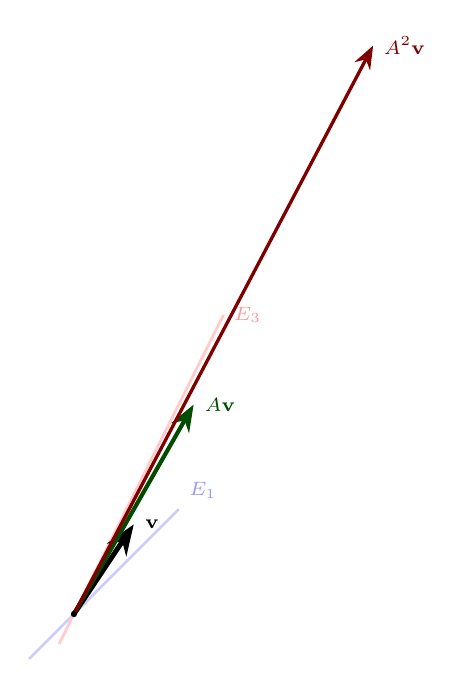
\begin{tikzpicture}[>=Stealth, scale=0.38]
  % Eigenspace lines
  \draw[blue!20, line width=1pt] (-1.5,-1.5) -- (3.5,3.5)
    node[above right, blue!40, font=\scriptsize] {$E_1$};
  \draw[red!20, line width=1pt] (-0.5,-1) -- (5,10)
    node[right, red!40, font=\scriptsize] {$E_3$};
  % n=0: v = (2,3) = (1,1)+(1,2)
  \draw[->, black, line width=1.8pt] (0,0) -- (2,3)
    node[right, font=\scriptsize] {$\mathbf{v}$};
  % n=1: Av = (4,7) = (1,1)+(3,6)
  \draw[->, black!70!green, line width=1.5pt] (0,0) -- (4,7)
    node[right, font=\scriptsize] {$A\mathbf{v}$};
  % n=2: A^2 v = (10,19) = (1,1)+(9,18)
  \draw[->, black!50!red, line width=1.2pt] (0,0) -- (10,19)
    node[right, font=\scriptsize] {$A^2\mathbf{v}$};
  \fill (0,0) circle (3pt);
\end{tikzpicture}
\end{center}

\vfill

Each step: the $E_3$ piece stretches $\times 3$, the $E_1$ piece is unchanged.

\vfill

\begin{center}
\fbox{\parbox{0.85\textwidth}{\centering
\x{Eigenvalues} tell you \x{how much} each direction stretches.\\[4pt]
\x{Eigenspaces} tell you \x{which} directions.\\[4pt]
Together, they completely describe what $A$ does.
}}
\end{center}

\end{frame}


% ┌─���───────────────────────────────────────────────────────────────────┐
% │ SECTION-LEVEL ADR: OUR RESTRICTION AND THE MINIMAL POLYNOMIAL      │
% │                                                                    │
% │ The standing assumption said distinct linear factors in det(tI-A). │
% │ But B from S3 had det(tI-B) = (t-2)^2(t-5) -- REPEATED root!     │
% │ Yet everything worked.                                             ���
% │                                                                    │
% │ The REAL restriction is about the MINIMAL polynomial, not the      │
% │ characteristic polynomial. min poly = lowest-degree annihilating   │
% │ polynomial. If it has distinct linear factors, everything works.   │
% │                                                                    │
% │ Non-example: J = [[2,1],[0,2]] has min poly (t-2)^2 -- repeated   │
% │ factor. Not enough eigenvectors. The shear.                        │
% └──────���─────────────────────────────────��────────────────────────────┘
\section{Our Restriction: The Minimal Polynomial}


% ADR: The tension -- B from S3 had a repeated char poly root.
% AUDIENCE EMOTION: "wait, our assumption said distinct factors!"
% AUDIENCE ATTENTION: the contradiction grabs attention.
\begin{frame}{A Repeated Root That Worked}

$B$ from \S3 had $\det(tI - B) = (t-2)^{\x{2}}(t-5)$ --- a \x{repeated} root!

\vfill

Yet the spectral machinery worked perfectly:
\begin{itemize}
\item Two distinct projections $P_2, P_5$ \;\checkmark
\item Compatible, partition of $I$ \;\checkmark
\item Cross-filling, eigenvectors \;\checkmark
\item $B = PDP^{-1}$ \;\checkmark
\end{itemize}

\vfill\pause

\x{Why?} The characteristic polynomial can repeat. What matters is a different polynomial.

\end{frame}


% ADR: Minimal polynomial definition. Lowest-degree monic poly that
% annihilates A. It divides every annihilating polynomial.
% AUDIENCE EMOTION: "there's a polynomial that controls everything"
% AUDIENCE ATTENTION: definition, then concrete example.
\begin{frame}{The Minimal Polynomial}

\begin{defi}[Minimal Polynomial]
The \x{minimal polynomial} $m(t)$ is the lowest-degree monic polynomial such that $m(A) = 0$.
\end{defi}

\vfill

It divides every annihilating polynomial (including $\det(tI - A)$).

\vfill\pause

\x{Check on $B$:}

$$(B - 2I)(B - 5I) = \begin{pmatrix}0&0&3\\0&0&3\\0&0&3\end{pmatrix}\begin{pmatrix}-3&0&3\\0&-3&3\\0&0&0\end{pmatrix} = \begin{pmatrix}0&0&0\\0&0&0\\0&0&0\end{pmatrix}$$

\vfill

So $m(t) = (t-2)(t-5)$ --- \x{distinct} linear factors. \;\checkmark

\end{frame}


% ADR: A = 3I_2 example -- char poly (t-3)^2 but min poly (t-3).
% AUDIENCE EMOTION: "even a scalar matrix is fine"
% AUDIENCE ATTENTION: extreme case, grounding.
\begin{frame}{Another Fine Example: $A = 3I$}

$$A = \begin{pmatrix}3&0\\0&3\end{pmatrix}, \qquad \det(tI - A) = (t-3)^2 \quad\text{(repeated!)}$$

\vfill

But $A - 3I = 0$ already, so $m(t) = t - 3$ \quad (degree 1, one distinct factor).

\vfill

Spectral decomposition: $A = 3 \cdot I$. Just one projection $P_1 = I$.

\vfill

The whole space $\mathbb{R}^2$ is one eigenspace. \quad Fine!

\end{frame}


% ADR: A case that needs new tools -- J = [[2,1],[0,2]].
% min poly = (t-2)^2, repeated factor. Eigenvectors span only a line.
% TikZ shows the shear: eigenvectors only on one line.
% Do NOT say "fail" or "cannot handle" -- say "needs new tools."
% AUDIENCE EMOTION: "there's something more to discover here"
% AUDIENCE ATTENTION: the shear diagram motivates future lectures.
\begin{frame}[shrink=5]{Beyond Our Assumption: The Shear}

$$J = \begin{pmatrix}2&1\\0&2\end{pmatrix}, \qquad \det(tI - J) = (t-2)^2$$

\vfill

$J - 2I = \begin{pmatrix}0&1\\0&0\end{pmatrix} \neq 0$. \qquad $(J - 2I)^2 = 0$.

\vfill

So $m(t) = (t-2)^2$ --- \x{repeated} factor!

\vfill\pause

\begin{center}
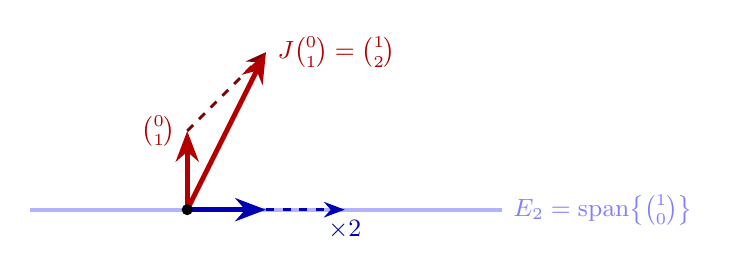
\begin{tikzpicture}[>=Stealth, scale=1.0]
  % Eigenspace line E_2
  \draw[blue!30, line width=1.5pt] (-2,0) -- (4,0)
    node[right, blue!50, font=\small] {$E_2 = \operatorname{span}\bigl\{\binom{1}{0}\bigr\}$};
  % On-eigenspace: scales by 2
  \draw[->, blue!70!black, line width=1.8pt] (0,0) -- (1,0);
  \draw[->, blue!70!black, line width=1pt, dashed] (1,0) -- (2,0)
    node[below, font=\small] {$\times 2$};
  % Off-eigenspace: shears
  \draw[->, red!70!black, line width=1.8pt] (0,0) -- (0,1)
    node[left, font=\small] {$\binom{0}{1}$};
  \draw[->, red!50!black, line width=1pt, dashed] (0,1) -- (1,2);
  \draw[->, red!70!black, line width=1.8pt] (0,0) -- (1,2)
    node[right, font=\small] {$J\binom{0}{1} = \binom{1}{2}$};
  \fill (0,0) circle (2pt);
\end{tikzpicture}
\end{center}

\vfill

Vectors on $E_2$ scale by 2. Vectors off $E_2$ get \x{sheared} --- not just scaled.

\vfill

This situation needs \x{new tools} --- a topic for a future lecture.

\end{frame}


% ADR: Summary of the restriction. Clean boxed statement.
% AUDIENCE EMOTION: "now I know the boundary"
% AUDIENCE ATTENTION: boxed takeaway.
\begin{frame}{The Real Restriction}

\vfill

\begin{center}
\fbox{\parbox{0.88\textwidth}{\centering
The characteristic polynomial CAN have repeated roots.\\[6pt]
The \x{minimal polynomial} is what matters:\\[8pt]
Distinct linear factors in $m(t)$ $\implies$ \x{diagonalizable}.\\[8pt]
Repeated factor in $m(t)$ $\implies$ needs new tools (future lecture).
}}
\end{center}

\vfill\pause

\begin{center}
\renewcommand{\arraystretch}{1.4}
\begin{tabular}{lcc}
 & Char.\ poly & Min.\ poly \\
\hline
$B = \left(\begin{smallmatrix}2&0&3\\0&2&3\\0&0&5\end{smallmatrix}\right)$ & $(t-2)^2(t-5)$ & $(t-2)(t-5)$ \quad\checkmark \\[4pt]
$3I_2$ & $(t-3)^2$ & $(t-3)$ \quad\checkmark \\[4pt]
$J = \left(\begin{smallmatrix}2&1\\0&2\end{smallmatrix}\right)$ & $(t-2)^2$ & $(t-2)^2$ \quad\x{$\boldsymbol\times$}
\end{tabular}
\end{center}

\end{frame}


% ┌─────────────────────────────────────────────────────────────────────┐
% │ SUMMARY AND PREVIEW                                                │
% └─────────────────────────────���───────────────────────────────────────┘
\section*{}


% ADR: Summary of the lecture. Key results in a compact boxed list.
% AUDIENCE EMOTION: "I can summarize this whole lecture in 4 lines"
% AUDIENCE ATTENTION: scannable, memorable.
\begin{frame}[shrink=5]{Summary}

\begin{enumerate}
\item $E_{\lambda_i} = \operatorname{Col}(P_i)$: eigenspace = column space of spectral projection.

\vspace{4pt}

\item Compatible projections (value tables verify instantly):
eigenvectors with different eigenvalues are independent; every vector decomposes uniquely.

\vspace{4pt}

\item Cross-fill $P_i = U_i V_i$: columns of $U_i$ = right eigenvectors,
rows of $V_i$ = left eigenvectors. $V_i U_j = \delta_{ij} I$.

\vspace{4pt}

\item Stack: $A = PDP^{-1}$, \; $g(A) = Pg(D)P^{-1}$ reduces every computation to plugging eigenvalues into $g$.

\vspace{4pt}

\item The \x{minimal polynomial} is the real restriction: distinct linear factors $\implies$ diagonalizable.
\end{enumerate}

\end{frame}


% ADR: Preview of next lecture.
% AUDIENCE EMOTION: "I wonder what happens with e^A"
% AUDIENCE ATTENTION: cliffhanger.
\begin{frame}{Next Lecture}

\vfill

We can compute $A^n$ via eigenvalues. But what about $e^A$?

\vfill

$$e^A = \lim_{n \to \infty}\left(I + \frac{A}{n}\right)^n$$

\vfill

\x{Next:} The exponential function, matrix exponential, and differential equations.

\vfill

\end{frame}


\end{document}
